\documentclass[a4paper, 12pt]{article}

%%%%%%%%%%%%
% Packages %
%%%%%%%%%%%%

\usepackage[french, english]{babel}

\usepackage[noheader]{packages/sleek}
\usepackage{packages/sleek-title}
\usepackage{packages/sleek-theorems}

%%%%%%%%%%%%%%
% Title-page %
%%%%%%%%%%%%%%

\logo{resources/pdf/logo-uliege.pdf}
\institute{University of Liège}
%\faculty{}
%\department{}
\title{Inverted Double Pendulum}
\subtitle{Optimal decision making for complex problems}
\author{%
Maxime \textsc{Meurisse} (s161278)\\%
François \textsc{Rozet} (s161024)%
}
%\supervisor{}
%\context{}
\date{Academic year 2020-2021}

%%%%%%%%%%%%%%%%
% Bibliography %
%%%%%%%%%%%%%%%%

\addbibresource{resources/bib/references.bib}

%%%%%%%%%%%%
% Document %
%%%%%%%%%%%%

\begin{document}
    \maketitle
    
    \section*{Introduction}
    
    In this project, we consider the \emph{Double Inverted Pendulum} control problem. We used this \href{https://github.com/benelot/pybullet-gym/blob/master/pybulletgym/envs/roboschool/envs/pendulum/inverted_double_pendulum_env.py}{source code}\footnote{We made a very little fix about camera settings. Our modified version of the library is provided in our archive. This modification does not affect the dynamics.} as a reference implementation of the environment.
    
    The Double Inverted Pendulum consists of two arms connected to each other by a hinge at their ends. One of the two arms is connected to a motorised cart, via a hinge, at its other end (Figure \ref{fig:domain.environment}).
    
    \begin{figure}[H]
        \centering
        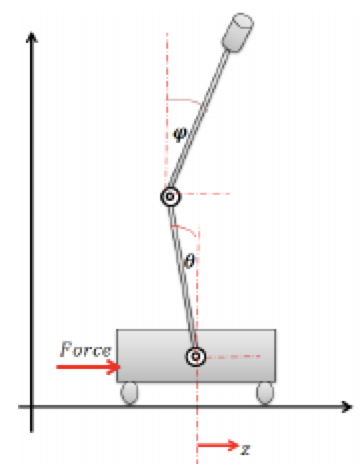
\includegraphics[width=0.35\textwidth]{resources/png/environment.png}
        \caption{The Double Inverted Pendulum environment.}
        \label{fig:domain.environment}
    \end{figure}
    
    This system is described by the displacement $z$ of the cart on a rail, along a single horizontal axis, and the position of each arm, respectively $\theta$ for the \enquote{first arm} and $\varphi$ for the \enquote{second arm}, relatively to their vertical position. The only input of the system is a force $F$ applied on the cart to move it along the rail.
    
    The goal is to keep the system, as long as possible, in a vertical position close, or similar, to the equilibrium position, \ie{} a situation where $\theta = \varphi = 0$.
    
    This system is under-actuated since the number of actuators is lower that the number of links: a single input force ($F$) in used to control the 3 degrees of freedom ($z$, $\theta$ and $\varphi$). Being unstable and chaotic, the Double Inverted Pendulum is among the most difficult problems to control. \cite{jadlovska2012classical, zhang2007fault}
    
    In this project, we try to stabilize the Double Inverted Pendulum using \emph{Reinforcement Learning} algorithms. The rest of this document is organized as follows: Section \ref{sec:domain} will formalize and characterize the environment and Section \ref{sec:policy.search.techniques} will explained our Reinforcement Learning algorithm (\emph{Deep Deterministic Policy Gradient} \cite{silver2014deterministic, lillicrap2015continuous}), evaluate its performance and compare it to a well-known algorithm (\emph{Fitted-Q-Iteration with Extremely Randomized Trees} \cite{ernst2005tree}) seen during the course.
    
    \newpage
    
    \section{Domain}\label{sec:domain}
    
    In this section, we define the dynamics of the system and give formalization and characterization of the environment.
    
    \subsection{Dynamics}
    
    The Double Inverted Pendulum as a continuous-time dynamics \cite{ernst2005tree}. Since it is very hard to infer the exact dynamics based on the reference source code we use, we referred to the dynamics described by \textcite{bogdanov2004optimal} instead.
    
    In the implementation we used, the dynamics has been discretized with the time between $t$ and $t + 1$ defined equal to $\SI{0.0165}{\second}$. An integration time step of $\SI{0.01}{\second}$ has been fixed.
    
    \subsection{Formalization and characterization}
    
    The system is \emph{deterministic}: when a force $F$ is applied to the cart, the latter and all other components react, without any randomness, according to their dynamics.
    
    To formalize the environment, we provide \emph{state space}, \emph{action space} and \emph{reward signal}.
    
    \subsubsection{State space}
    
    As mentioned in the introduction, the environment has three degrees of freedom: $z$, $\theta$ and $\varphi$. It can then be fully described by a state $\bm{x}\in\mathbb{R}^6$,
    \begin{equation}
        \bm{x} = \begin{pmatrix}
            z & \dot{z} & \theta & \dot{\theta} & \varphi & \dot{\varphi}
        \end{pmatrix}^T
    \end{equation}
    where $\dot{\square}$ denotes the derivative of $\square$. The derivatives give velocities, respectively of the cart, the first arm and the second arm, which are necessary to describe the state without ambiguity. Indeed, for a given position, an element can be moving to the left, to the right or stay still.
    
    The displacement $z$ is a continuous value belonging to the interval $[-1, +1]$ (with $-1$ corresponding to the left most position, and $+1$ the right most one) representing the displacement of the cart on a rail, relative to the center position $0$.
    
    Each angle can take any value between $-\pi$ and $+\pi$. However, one should note that, in practice, a wide range of angle values can never be reached by the system since the simulation is stopped when it reaches a terminal state (defined later in this Section).
    
    In the implementation of the environment we used, the agent doesn't have direct access to these values. Instead, the agent receives an \emph{observation} $o(\bm{x}) \in \mathbb{R}^9$ of the state,
    \begin{equation}
        o(\bm{x}) = \begin{pmatrix}
            z & \dot{z} & p_x & \sin\theta & \cos\theta & \dot{\theta} & \sin\varphi & \cos\varphi & \dot{\varphi}
        \end{pmatrix}^T
    \end{equation}
    where $p_x$ is the the displacement of the second arm's center of mass, in the same coordinate system as $z$.
    
    The system starts in an \emph{initial state} defined by setting the displacement $z$ to $0$ and the position of each arm's center of mass, along the horizontal axis, to a value drawn from $\mathcal{U}([-0.1, 0.1])$. The velocity (and torque) of each arm is initially set to $0$.
    
    The simulation stops when a \emph{terminal state} is reached. A state is considered as terminal when $p_y$, the second arm's center of mass position along the vertical axis, is lower or equal to a fixed threshold $\tau = \num{0.7}$.
    
    \subsubsection{Action space}
    
    The system only has one action $u$ that correspond to the force $F$ applied on the cart.
    
    The action $u$ is a continuous value belonging to the interval $U = [-1, 1]$. At each step of the simulation, the value of $u$ is injected in the system dynamics to move the cart.
    
    Depending of the sign of $u$, the cart accelerates to the left (negative value) or to the right (positive value).
    
    \subsubsection{Reward signal}
    
    The \emph{reward signal} $r$ is defined as a sum of three terms,
    \begin{equation}\label{eq:reward.signal}
        r(\bm{x}) = R_a - r_d(\bm{x}) - R_v
    \end{equation}
    where
    
    \begin{itemize}
        \item $R_a$ is a constant reward equal to $\num{10}$ that the agent receives at each step for being still alive;
        \item $r_d(\bm{x})$ is defined as
        \begin{equation}
            r_d(\bm{x}) = \frac{1}{100}p_x^2 + (p_y - \num{1.7})^2
        \end{equation}
        with $p = (p_x, p_y)$ the position of the second arm's center of mass;
        \item $R_v$ is a constant reward equal to $\num{0}$.
    \end{itemize}
    
    \begin{note}
        Normally, the term $R_v$ is computed using velocity of each hinge so that the higher the velocity of each hinge, the more the agent is penalised. However, in the implementation we used, this term is manually set to $\num{0}$ due to an issue in the code. Therefore, there is no penalty for having arms that move too fast.
    \end{note}
    
    Therefore, at each step of the simulation, the agent receives a reward that depends mainly on the position of its second arm: the closer the arm is to its vertical equilibrium position, the higher the reward will be.
    
    \newpage
    
    \section{Policy Search Techniques}\label{sec:policy.search.techniques}
    
    In this section, we first implement the \emph{Deep Deterministic Policy Gradient} (DDPG) algorithm \cite{lillicrap2015continuous} as a policy search technique.

    Then, we implement a well-known algorithm seen during the course: the \emph{Fitted-Q-Iteration with Extremely Randomized Trees} (FQI with XRT) \cite{ernst2005tree}.
    
    Finally, we evaluate and compare policies obtained in terms of \emph{expected discounted cumulative reward} obtained at the end of each episode.
    
    \begin{note}
        For the sake of simplicity, in the rest of this Section, the observation $o(\bm{x})$ of the agent will be simply noted as $x$ and be qualified as its \enquote{state}.
    \end{note}
    
    \subsection{Deep Deterministic Policy Gradient}
    
    \emph{The explanations provided in this section are inspired by \cite{silver2014deterministic, lillicrap2015continuous, ddpgopenai, ddpgtds, bollandinfo80031, bollandinfo80032}}.
    
    While \emph{Q-learning} and \emph{Deep Q-learning} (DQL) were particularly well suited for our previous assignments with discrete action spaces, they can not be used in the Double Inverted Pendulum problem since the action space is continuous. For this reason, we decide to work with the DDPG algorithm, which is a kind of adaptation of DQL to continuous action spaces.
    
    The DDPG algorithm is shown in Algorithm \ref{alg:ddpg}. The main steps is explained in the following.
    
    \begin{algorithm}[h]
        \begin{algorithmic}[1]
            \State{Initialize policy parameter $\theta$, $Q$-function parameters $\phi$, empty replay buffer $\mathcal{D}$}
            \State{Set target parameters equal to main parameters: $\theta_{\text{targ}} \leftarrow \theta$, $\phi_{\text{targ}} \leftarrow \phi$}
            \Repeat
                \State{Observe $x$ and select $u = \min \cbk{ \max \cbk{\mu_\theta(x) + \varepsilon, u_{Low}}, u_{High}}$} \label{alg:action.selection}
                \State{Execute $u$} \label{alg:ddpg.execute}
                \State{Observe next state $x'$, reward $r$ and done signal $d$} \label{alg:ddpg.observe}
                \State{Store $(x, u, r, x', d)$ in $\mathcal{D}$} \label{alg:ddpg.store}
                \If{$x'$ is terminal}
                    \State{Reset environment state}
                \EndIf
                \If{it's time to update} \label{alg:ddpg.update.time}
                    \For{however many updates} \label{alg:ddpg.updates}
                        \State{Randomly sample a batch $B$ of transitions from $\mathcal{D}$} \label{alg:ddpg.sample}
                        \State{Compute targets
                        \begin{equation}
                            y(r, x', d) = r + \gamma(1 - d)Q_{\phi_{\text{targ}}}(x', \mu_{\theta_{\text{targ}}}(x'))
                        \end{equation}
                        }
                        \State{Update Q-function by one step of gradient descent using
                        \begin{equation}
                            \nabla_{\phi} \frac{1}{|B|} \sum_{(x, u, r, x', d) \in B}(Q_{\phi}(x, u) - y(r, x', d))^2
                        \end{equation}
                        }
                        \State{Update policy by one step of gradient ascent using
                        \begin{equation}
                            \nabla_{\theta} \frac{1}{|B|} \sum_{x \in B} Q_{\phi}(x, \mu_{\theta}(x))
                        \end{equation}
                        }
                        \State{Update target networks with
                        \begin{align}
                            \phi_{\mathrm{targ}} & \leftarrow \rho \phi_{\mathrm{targ}} + (1-\rho) \phi\label{eq:polyak.update.phi}\\
                            \theta_{\mathrm{targ}} & \leftarrow \rho \theta_{\mathrm{targ}} + (1-\rho) \theta\label{eq:polyak.update.theta}
                        \end{align}
                        }
                    \EndFor
                \EndIf
            \Until{convergence}
        \end{algorithmic}
        \caption{Deep Deterministic Policy Gradient \cite{ddpgopenai, lillicrap2015continuous}}
        \label{alg:ddpg}
    \end{algorithm}
    
    \subsubsection{Neural networks}
    
    The DDPG algorithm uses four neural networks: a deterministic policy function network $\theta$, a $Q$-network $\phi$ and two target networks associated to, respectively, $\theta$ and $\phi$. Networks $\theta$ and $\phi$ acts like \emph{Advantage Actor-Critic} \cite{sutton2018reinforcement}: the actor ($\theta$) chooses an action at each time step and the critic ($\phi$) evaluates the quality of the $Q$-value.
    
    Target networks are time-delayed copies of original networks. Their use helps to improve stability during training, as already explained in our Assignment 3.
    
    Each network is a shallow \emph{Multi-Layer Perceptron} (MLP) with an input layer, one hidden layer composed of $256$ neurons and an output layer. All activation functions are ReLU. The output of the actor network passes trough a $\tanh$ activation function.
    
    For both networks, we use an Adam \cite{kingma2014adam} optimizer with learning rates set to, respectively, $\num{e-4}$ and $\num{e-3}$.
    
    Target networks are updated using \emph{Polyak averaging} \cite{polyak1992acceleration} at the end of each update step (\emph{cf.} equations \ref{eq:polyak.update.phi} and \ref{eq:polyak.update.theta}). We fixed the value of $\rho$ to $\num{e-2}$.
    
    \subsubsection{Action selection}
    
    Each action is selected using the policy network (line \ref{alg:action.selection} of the Algorithm). Exploration is done by adding a noise $\varepsilon$ directly to the action selected.
    
    To generate the noise $\varepsilon$, we use the same process as \textcite{lillicrap2015continuous}: the \emph{Ornstein–Uhlenbeck process}. The latter generates a sequence of noises $\varepsilon_i$ which are correlated. The exact relation is
    \begin{equation}\label{eq:orstein-uhlenbeck}
        \varepsilon_{i+1} = \varepsilon_i + a(b - \varepsilon) + c \mathcal{N}(0, 1)
    \end{equation}
    with $\varepsilon_0$ drawn from $\mathcal{N}(0, 1)$. We set $a$, $b$ and $c$ to, respectively, $\num{0.15}$, $\num{0}$ and $\num{0.2}$.
    
    \subsubsection{Replay buffer}
    
    As for Deep Q-learning implemented in our previous Assignment 3, we use a replay buffer $\mathcal{D}$ of capacity $\num{65536}$. We fill the buffer by adding transitions collected during episode simulations (line \ref{alg:ddpg.execute}, \ref{alg:ddpg.observe} and \ref{alg:ddpg.store} of the Algorithm). A transition is a tuple $(x, u, r, x', d)$ where $x$ is the state of the agent, $u$ the action played, $r$ the reward, $x'$ the new state and $d$, the \emph{done signal}, a binary value indicating whether the agent has reach a terminal state ($1$) or not ($0$).
    
    When the buffer contains enough elements, we sample batches of $\num{32}$ elements (line \ref{alg:ddpg.sample} of the Algorithm) to train the networks. An update of the networks (line \ref{alg:ddpg.update.time} of the Algorithm) is done after each step of an episode (line \ref{alg:ddpg.updates} of the Algorithm), when the buffer contains enough elements.
    
    \subsubsection{Discrete action space}
    
    DDPG algorithm is, by default, no suitable for discrete action space. To adapt it, we use the \emph{Wolpertinger policy} \cite{dulac2015deep}.
    
    This policy can be seen as additional steps added to the action selection of the Algorithm \ref{alg:ddpg} (line \ref{alg:action.selection}). Firstly, we define a discrete action space $U_d$. Secondly, we use the Actor network to get a (continuous) action $u$. Instead of directly using $u$, we give it to a \emph{$k$ nearest neighbors} model that outputs $k$ nearest discrete actions $u_{d_i} \in U_d$ (with $i = 1, \dots, k$). Finally, we create all $(x, u_{d_i})$ pairs, with $x$ being the current state of the agent, and keep the action associated to the pair that maximize the $Q$-value approximated by the Critic network.
    
    In our project, we set $k$ to half the number of discrete actions. It is important to note that, in the case of discrete action space, we do not add noise $\varepsilon$ to the selected discrete action.
    
    \begin{note}
        As mentioned in the original paper \cite{dulac2015deep}, the Wolpertinger policy has been designed for \emph{large} discrete action spaces. In our project, working with $k$ nearest neighbors of a continuous action or with all discretized actions doesn't make much difference because $U_d$ is very small. Still, we choose to work with the Wolpertinger policy to have a more general algorithm.
        
        Moreover, to get the nearest neighbors, we work with a $k$ nearest neighbors model from the \href{https://scikit-learn.org/}{scikit-learn} library. Our action space being one-dimensional, this model is overly complex for the task, but, once again, we keep it in order to have a more general implementation.
    \end{note}
    
    \subsection{Fitted-Q-Iteration with Extremely Randomized Trees}
    
    \emph{The content of this Section is inspired from our previous Assignment 2.}
    
    We choose to compare performance of the DDPG algorithm with the FQI with XRT algorithm seen during the course.
    
    The goal of the FQI algorithm is to train a sequence of supervised regressors $\hat{Q}_1$, $\hat{Q}_2$, \dots, $\hat{Q}_N$ estimating respectively the functions $Q_1$, $Q_2$, \dots, $Q_N$. To do so, $N$ training sets are built. Let $h_i$ ($i = 1, \ldots, N$) be sets of one-step transitions $\cbk{(x_k, u_k, r_k, x'_k) \mid k = 1, \ldots, t}$. Then, the training sets are
    \begin{align*}
        \text{TS}_1 & = \cbk{\rbk{(x, u), r} \mid (x, u, r, x') \in h} \\
        \text{TS}_i & = \cbk{\rbk{(x, u), r + \gamma \max _{u' \in U} \hat{Q}_{i - 1}(x', u')} \mid (x, u, r, x') \in h_i } \quad \forall i \geq 2
    \end{align*}
    and $\hat{Q}_i$ is trained on $\text{TS}_i$.
    
    We use our implementation of Assignment 2 and adapt it to the Double Inverted Pendulum control problem. More precisely,
    
    \begin{enumerate}
        \item We compute $N$ using
        \begin{equation}
            N = \left\lceil \log_{\gamma} \rbk{\frac{\epsilon}{2 B_r}(1-\gamma)^2} \right\rceil .
        \end{equation}
        By fixing $\gamma$ to $\num{0.95}$, $\epsilon$ to $\num{1}$\footnote{We considered this precision to be sufficient as it is numerically insignificant with respect to the cumulative rewards, \cf{} Section \ref{sec:performances.comparisons}.} and $B_r$ to $\num{10}$ (maximum possible value of \eqref{eq:reward.signal}), we get $N = \num{176}$.
        \item\label{itm:h1} We create $h_1$ by generating and storing $\num{3000}$ transitions using a random policy.
        \item For all values $i$ from $1$ to $N$,
        \begin{enumerate}
            \item We train the model (XRT) using all stored transitions ($h_i$) to get $\hat{Q}_i$.
            \item\label{itm:fqi.evaluation} We play $20$ episodes to evaluate $\hat{Q}_i$ and save all new transitions obtained.
            \item We create a new training set by appending all new transitions to current transitions stored. More formally, let $h_e$ be the transitions collected during evaluation. The new training set $h_{i+1}$ is defined as
            \begin{equation}
                h_{i+1} = h_i \cup h_e
            \end{equation}
            with $h_1$ defined in step \ref{itm:h1} of the algorithm.
        \end{enumerate}
    \end{enumerate}
    
    \subsection{Performances and comparisons}\label{sec:performances.comparisons}
    
    In this section, we compare performances of our algorithms. To do this, at the end of each optimization step, we play some trajectories ($50$ for DDPG, $20$\footnote{We do not play $50$ trajectories for FQI because it adds too much new transitions and therefore greatly increases the training time of the model.} for FQI, \cf{} step \ref{itm:fqi.evaluation} of the algorithm) and compute, for each trajectory $i$, the \emph{discounted cumulative reward} $C$ using
    \begin{equation}
        C_i = \sum_{t=0}^{T-1} \gamma^t r_{i, t}
    \end{equation}
    where $T$ is the (maximum) number of steps in a trajectory. We then compute the \emph{expected discounted cumulative reward} $J^{\mu}$ by computing the mean of all $C_i$, \ie{}
    \begin{equation}
        J^{\mu} = \frac{1}{n}\sum_{i=0}^{n-1}C_i
    \end{equation}
    with $n$ being the number of trajectories played. We also compute the standard deviation $\sigma$ of all $C_i$. In the following, each graph presented shows $J^{\mu}$ as a thick blue line and $J^{\mu} \pm \sigma$ as a lighter blue area around the line.
    
    For both algorithms, we set $\gamma$ to $\num{0.95}$.
    
    \subsubsection{DDPG}
    
    We played $\num{500}$ episodes with a maximum number of steps fixed to $T = \num{1000}$. In the discrete action space case, we use $11$ discretized actions that are linearly spaced in the interval $[-1, 1]$. We choose an odd number of actions to be sure that the action \enquote{$0$} (no force is applied) is available. The obtained results are shown in Figure \ref{fig:ddpg.rewards}.
    
    \begin{figure}[H]
        \centering
        \begin{subfigure}{0.49\textwidth}
            \centering
            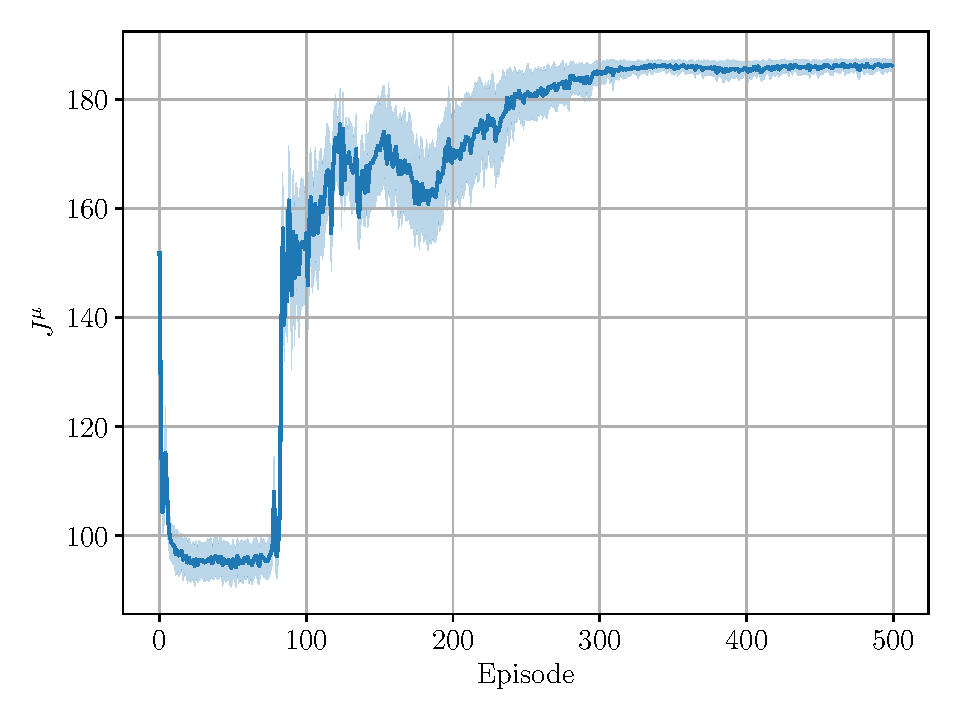
\includegraphics[width=\textwidth]{resources/pdf/ddpg_J_None_1_0.95.pdf}
            \caption{Continuous action space.}
        \end{subfigure}
        \hfill
        \begin{subfigure}{0.49\textwidth}
            \centering
            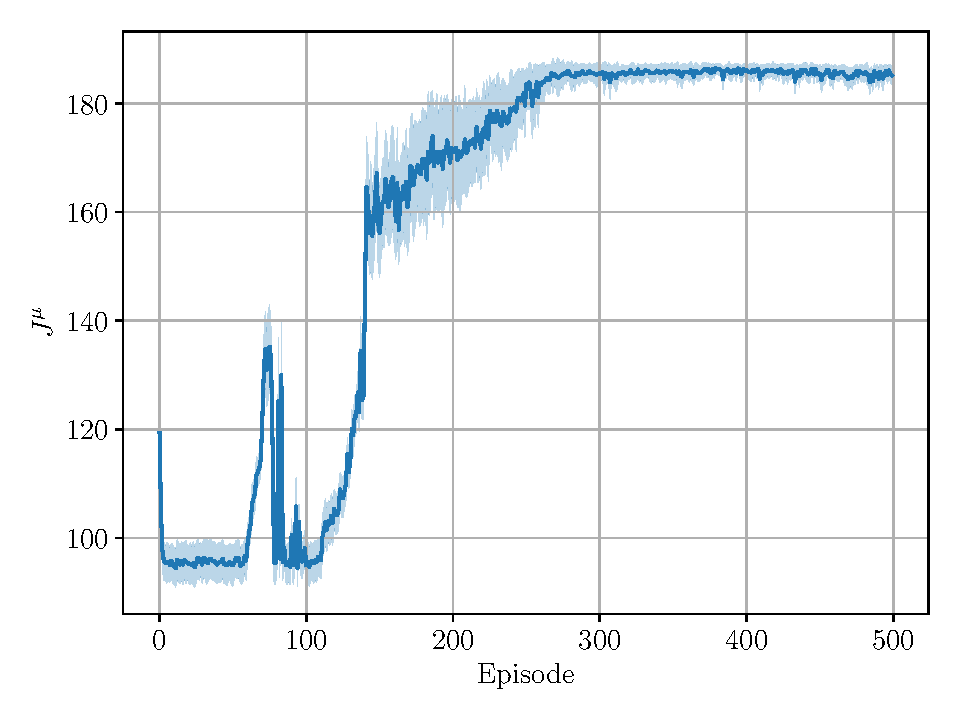
\includegraphics[width=\textwidth]{resources/pdf/ddpg_J_11_1_0.95.pdf}
            \caption{Discrete action space.}
        \end{subfigure}
        \caption{Expected discounted cumulative rewards of DDPG algorithm.}
        \label{fig:ddpg.rewards}
    \end{figure}
    
    We observe that, for both continuous and discrete action spaces, the algorithms converge, after approximately $\num{300}$ episodes, to an expected discounted cumulative reward of approximately $\num{190}$. Once the algorithms have converged, it seems to stabilize and do not evolve anymore over time.
    
    Except at the beginning, we do not note significant differences in results obtained between continuous and discrete action spaces.
    
    We also judge the quality of our policy by visually checking the simulation. Although the agent does not remain in equilibrium for long, it clearly improves over time, moving from an anarchic policy to one that allows it to remain in equilibrium for a short period of time.
    
    \paragraph{Neural networks depths}
    
    By default, we use very shallow neural networks for Actor and Critic. We try to use deeper ones to see the influence. We use, for both Actor and Critic, $8$ hidden layers of $256$ neurons and ELU \cite{clevert2015fast} activation function. The obtained results are shown in Figure \ref{fig:ddpg.rewards.deeper}.
    
    \begin{figure}[H]
        \centering
        \begin{subfigure}{0.49\textwidth}
            \centering
            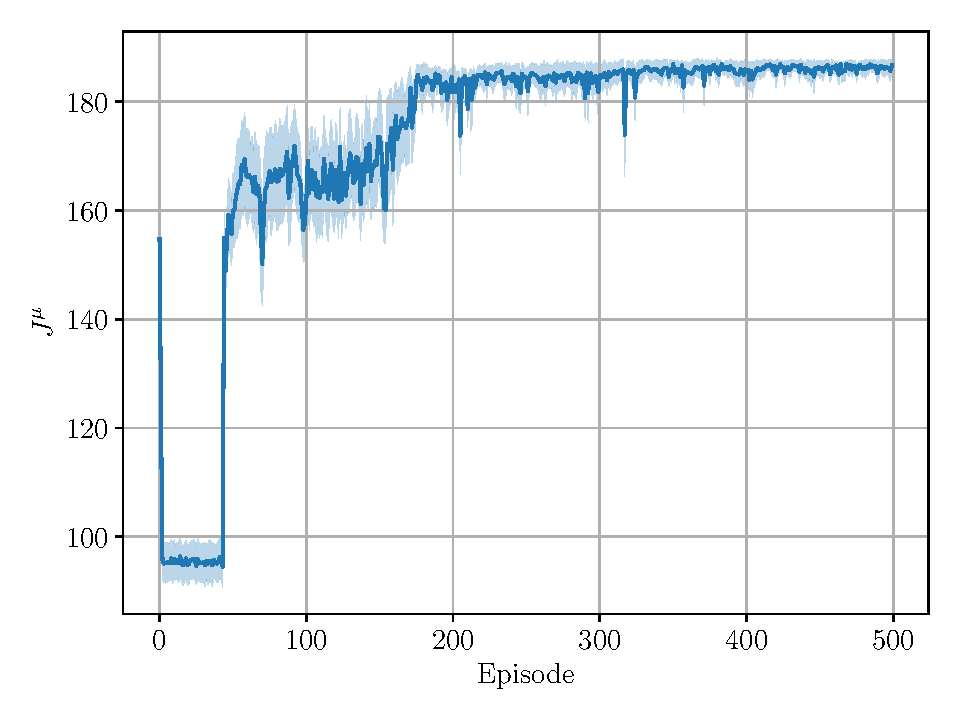
\includegraphics[width=\textwidth]{resources/pdf/ddpg_J_None_8_0.95.pdf}
            \caption{Continuous action space.}
        \end{subfigure}
        \hfill
        \begin{subfigure}{0.49\textwidth}
            \centering
            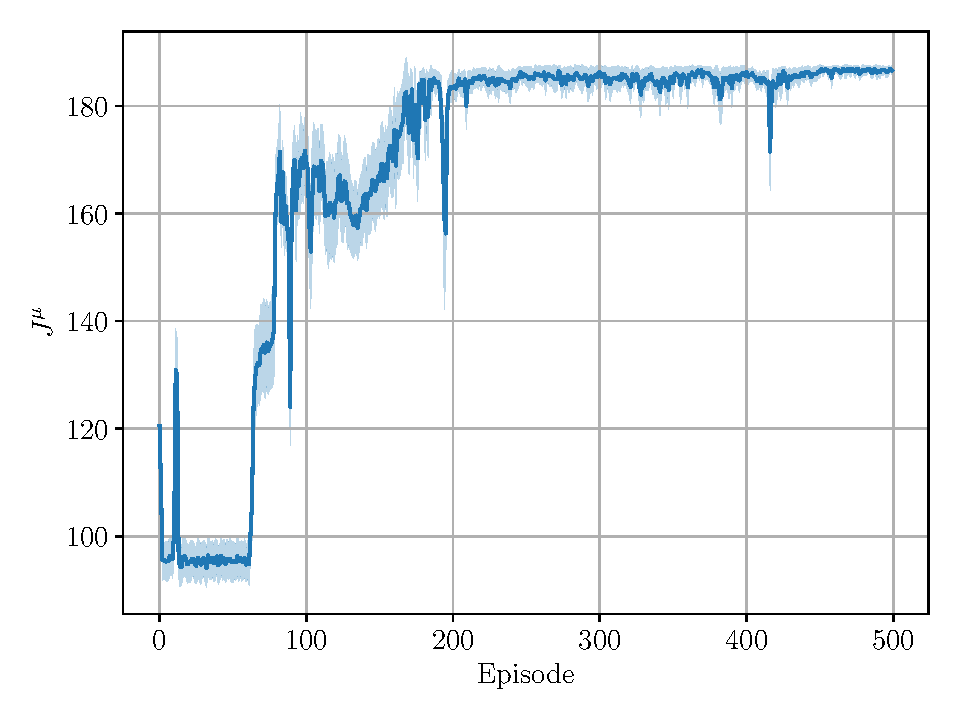
\includegraphics[width=\textwidth]{resources/pdf/ddpg_J_11_8_0.95.pdf}
            \caption{Discrete action space.}
        \end{subfigure}
        \caption{Expected discounted cumulative rewards of DDPG algorithm using deeper neural networks.}
        \label{fig:ddpg.rewards.deeper}
    \end{figure}
    
    We observe that the algorithms converge to the same $J^{\mu}$, but faster: only $\num{200}$ episodes is needed to reach such a value.
    
    \paragraph{Discrete action space size}
    
    We try to reduce the number of discretized actions in the case of a discrete action space. We choose two odd numbers ($7$ and $5$) generated in the same way as previously. The results are shown in Figure \ref{fig:ddpg.rewards.size}.
    
    \begin{figure}[H]
        \centering
        \begin{subfigure}{0.49\textwidth}
            \centering
            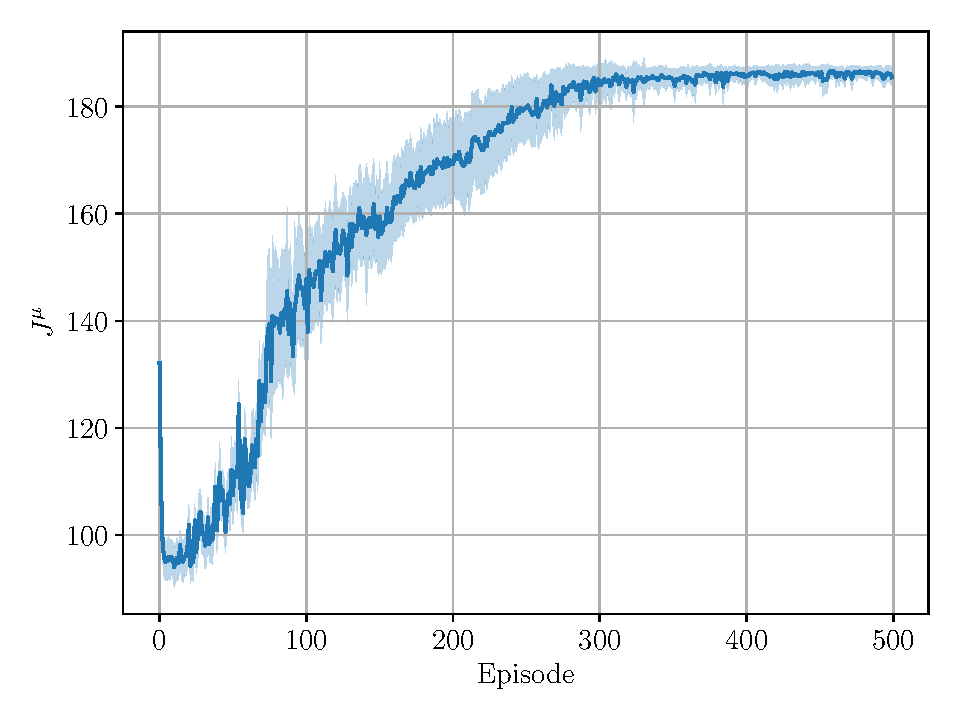
\includegraphics[width=\textwidth]{resources/pdf/ddpg_J_7_1_0.95.pdf}
            \caption{$7$ discretized actions.}
        \end{subfigure}
        \hfill
        \begin{subfigure}{0.49\textwidth}
            \centering
            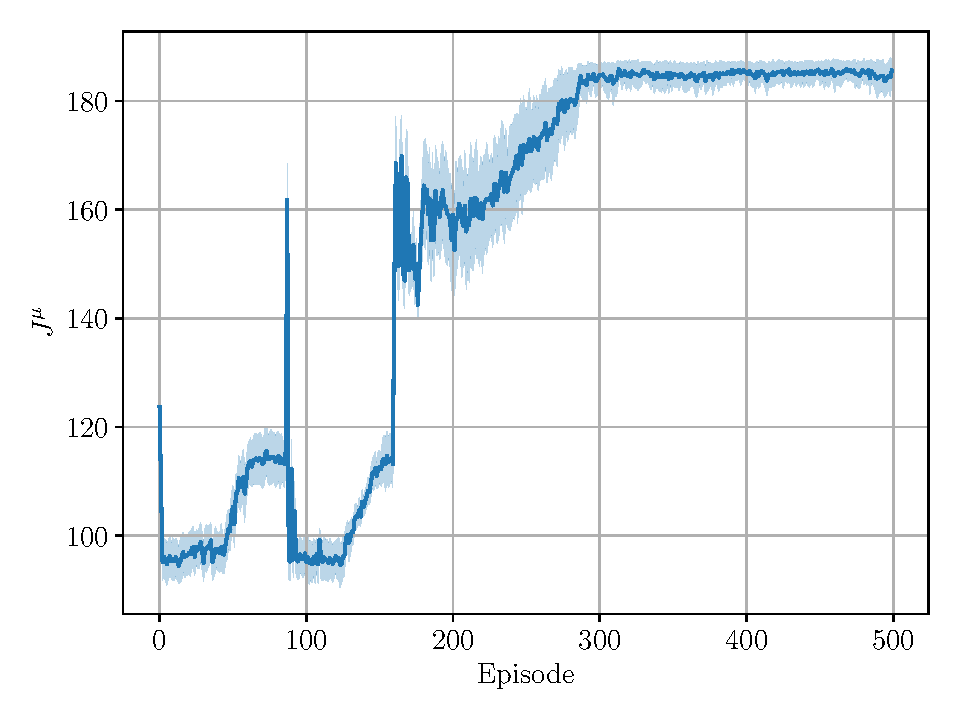
\includegraphics[width=\textwidth]{resources/pdf/ddpg_J_5_1_0.95.pdf}
            \caption{$5$ discretized actions.}
        \end{subfigure}
        \caption{Expected discounted cumulative rewards of DDPG algorithm with different action space sizes.}
        \label{fig:ddpg.rewards.size}
    \end{figure}
    
    We observe that, in both cases, the agent still learns a good policy. However, the convergence of $J^{\mu}$ with $7$ actions is smoother, and slightly faster, than the convergence with $5$ actions. It can be explained by the fact that, in view of the complexity of the problem, the fewer actions available, the more difficult it will be for the agent to learn. To verify this fact, we train the agent with $3$ discretized actions (\cf{} Figure \ref{fig:ddpg.rewards.size.3}).
    
    \begin{figure}[H]
        \centering
        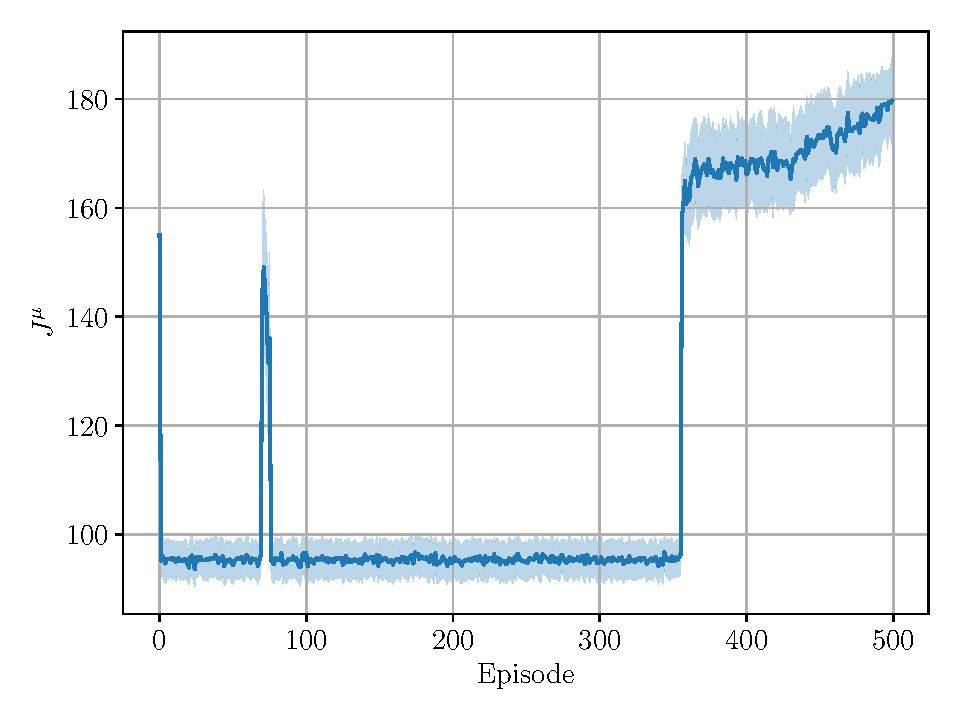
\includegraphics[width=0.6\textwidth]{resources/pdf/ddpg_J_3_1_0.95.pdf}
        \caption{Expected discounted cumulative rewards of DDPG algorithm with $3$ discretized actions.}
        \label{fig:ddpg.rewards.size.3}
    \end{figure}
    
    We observe that, as expected, the agent has more difficulty to learn a good policy. The values of $J^{\mu}$ start to improve after $\num{350}$ episodes and only reaches $\num{180}$ after $\num{500}$ episodes.
    
    \subsubsection{FQI with XRT}
    
    We train our model (XRT with $20$ estimators) until $N = \num{176}$. We fixed the maximum number of steps to $T = \num{1000}$. We use $11$ discretized actions linearly spaced in the interval $[-1, 1]$. The results are shown in Figure \ref{fig:fqi.xrt.rewards}.
    
    \begin{figure}[H]
        \centering
        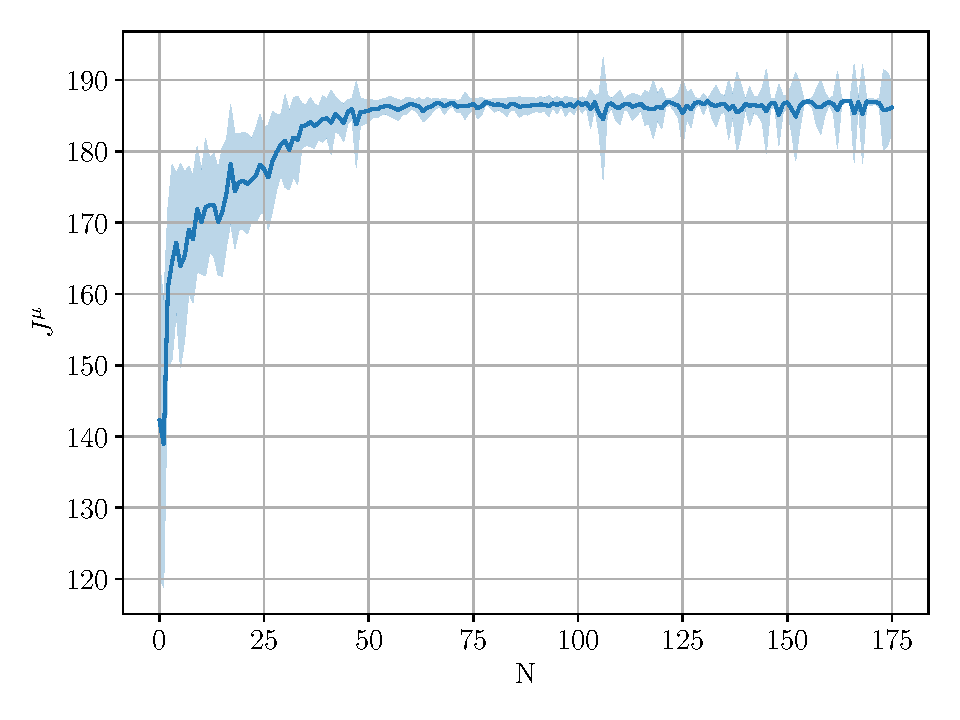
\includegraphics[width=0.6\textwidth]{resources/pdf/fqi_J_11_20.pdf}
        \caption{Expected discounted cumulative reward of FQI with XRT algorithm.}
        \label{fig:fqi.xrt.rewards}
    \end{figure}
    
    We observe that the algorithm converge, after $N \approx \num{47}$, to a $J^{\mu}$ slightly below $\num{190}$, as for DDPG algorithm.
    
    \subsubsection{Comparison}
    
    All algorithms implemented (DDPG in continuous and discrete action spaces and FQI with XRT) seem to converge and learn a policy that allows to stabilize, for a short amount of time, the pendulum. While FQI with XRT seems to converge faster than DDPG, the latter is faster to train. It can be explained by the fact that FQI is trained on all transitions stored (that grows during the training. To give an idea, at the last optimization step, the transition list contains $\num{601237}$ transitions.) while DDPG is trained with random batches of the same size regardless of how many episodes have passed.
    
    \subsection{Possible improvements}
    
    Our algorithms could be improved on several aspects.
    
    Concerning the DDPG algorithm, we could make the sampling of an action more complex. For the moment, in our implementation of the Ornstein-Uhlenbeck process, \ie{} \eqref{eq:orstein-uhlenbeck}, the variance of $\mathcal{N}$ is fixed at $1$. We could, for example, modify the Actor neural network so that it returns an action $u$ and a variance $\sigma^2$ and uses the latter in the noise generation process.
    
    We also used, in our implementation, a replay buffer that randomly samples batches of data at each optimization step. An interesting work by \textcite{hou2019improving} has shown that working with a \emph{Prioritized Replay Buffer} can improve results in term of training time, robustness and final performance.
    
    Other improvements to the DDPG algorithm are also possible \cite{mediumddpgimprovements}: \emph{Asynchronous Advantage Actor-Critic} \cite{mnih2016asynchronous} that takes advantage of multiple Actor networks trained in parallel, or \emph{Distributed Distributional Deterministic Policy Gradients} \cite{barth2018distributed} that works with multiple independent Actors, prioritized replay buffer and distributional Critic.
    
    Concerning the FQI algorithm, we could reduce the number of transitions used to train the model and thereby reduce the training time. As the transitions generated at the beginning progressively lose their relevance as the training progresses, we could, for example, work with a cyclic buffer of fixed capacity. Thus, when the maximum capacity is reached, the oldest transitions are replaced by new ones and the dataset size remains constant.

    \newpage

    \printbibliography
\end{document}
